\documentclass[tikz,border=2pt]{standalone}
\usepackage[T1]{fontenc}
\usepackage{helvet,amsmath,amssymb,fix-cm}
\renewcommand{\familydefault}{\sfdefault}
\usetikzlibrary{arrows.meta,calc,positioning,fit,backgrounds,decorations.pathreplacing,shapes.geometric}
\definecolor{ink}{HTML}{243343}
\definecolor{physical}{HTML}{3478A3}
\definecolor{semantic}{HTML}{B27C26}
\definecolor{feasible}{HTML}{248679}
\definecolor{decode}{HTML}{75609D}
\definecolor{fault}{HTML}{BA5554}
\definecolor{muted}{HTML}{6F7D88}
\tikzset{
  every node/.style={font=\fontsize{9}{10.8}\selectfont,text=ink},
  edge/.style={-{Stealth[length=1.8mm,width=1.25mm]},line width=.6pt,draw=ink},
  param/.style={-{Stealth[length=1.7mm]},line width=.6pt,draw=decode,dashed},
  link/.style={line width=.8pt,draw=physical},
  reject/.style={line width=.7pt,draw=fault,dashed},
  panel/.style={rounded corners=2pt,draw=muted!45,line width=.45pt,fill=white},
  box/.style={rounded corners=2pt,draw=physical!70,line width=.55pt,fill=physical!6,align=center,inner sep=3pt},
  sem/.style={box,draw=semantic!70,fill=semantic!8},
  gate/.style={box,draw=feasible!70,fill=feasible!7},
  dec/.style={box,draw=decode!70,fill=decode!7},
  tinylabel/.style={font=\fontsize{8}{9.4}\selectfont},
  smalllabel/.style={font=\fontsize{8.5}{10}\selectfont},
  heading/.style={font=\bfseries\fontsize{10}{11.5}\selectfont,anchor=north west},
  dot/.style={circle,minimum size=.43cm,inner sep=0pt,draw=physical,fill=white,line width=.8pt,font=\bfseries\fontsize{9}{10}\selectfont},
  receiver/.pic={\draw[draw=physical,line width=.8pt] (0,0)--(0,.58) (-.17,0)--(.17,0) (-.15,.39)--(0,.58)--(.15,.39);
    \draw[draw=physical!70,line width=.55pt] (-.2,.56) arc[start angle=160,end angle=200,radius=.23];
    \draw[draw=physical!70,line width=.55pt] (.2,.40) arc[start angle=-20,end angle=20,radius=.23];},
}
\begin{document}
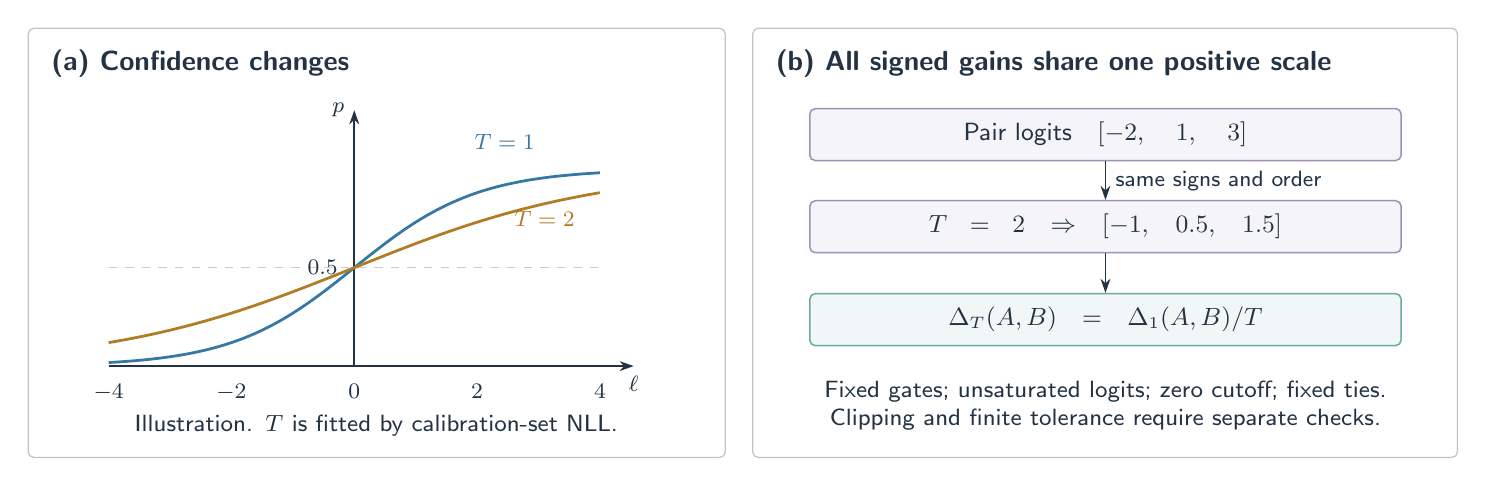
\begin{tikzpicture}[x=1cm,y=1cm]
\draw[panel] (0,0) rectangle ++(8.85,5.45);
\node[heading] at (0.17,5.3) {(a) Confidence changes};
\draw[panel] (9.2,0) rectangle ++(8.95,5.45);
\node[heading] at (9.37,5.3) {(b) All signed gains share one positive scale};

\begin{scope}[shift={(1.02,1.16)},x=.78cm,y=2.50cm]
\draw[edge] (-.0,0)--(8.55,0) node[below,tinylabel] {$\ell$};
\draw[edge] (4,0)--(4,1.3) node[left,tinylabel] {$p$};
\draw[muted!40,dashed] (0,.5)--(8,.5);
\node[tinylabel,anchor=east] at (3.89,.5) {$0.5$};
\foreach \xx/\lab in {0/-4,2/-2,4/0,6/2,8/4} \node[tinylabel,anchor=north] at (\xx,-.04) {$\lab$};
\draw[physical,line width=1pt,domain=0:8,samples=81] plot (\x,{1/(1+exp(-(\x-4)))});
\draw[semantic,line width=1pt,domain=0:8,samples=81] plot (\x,{1/(1+exp(-(\x-4)/2))});
\node[tinylabel,text=physical,anchor=west] at (5.8,1.14) {$T=1$};
\node[tinylabel,text=semantic,anchor=west] at (6.45,.75) {$T=2$};
\end{scope}
\node[smalllabel,align=center,text width=7.8cm] at (4.42,.40)
 {Illustration. $T$ is fitted by calibration-set NLL.};
\node[dec,text width=7.30cm,minimum height=.66cm] (ell) at (13.68,4.10)
 {Pair logits\quad $[-2,\;1,\;3]$};
\node[dec,text width=7.30cm,minimum height=.66cm] (scaled) at (13.68,2.93)
 {$T=2$\quad $\Rightarrow$\quad $[-1,\;0.5,\;1.5]$};
\draw[edge] (ell)--node[right,tinylabel] {same signs and order} (scaled);
\node[gate,text width=7.30cm,minimum height=.66cm] (gain) at (13.68,1.75)
 {$\Delta_T(A,B)=\Delta_1(A,B)/T$};
\draw[edge] (scaled)--(gain);
\node[smalllabel,align=center,text width=7.8cm] at (13.68,.66)
 {Fixed gates; unsaturated logits; zero cutoff; fixed ties.\\Clipping and finite tolerance require separate checks.};
\end{tikzpicture}
\end{document}
